\documentclass{article}
\linespread{1.3}
\usepackage[margin=50pt]{geometry}
\usepackage{amsmath, amsthm, amssymb, amsthm, tikz, fancyhdr}
\pagestyle{fancy}
\renewcommand{\headrulewidth}{0pt}
\newcommand{\changefont}{\fontsize{15}{15}\selectfont}

\newcommand{\field}[1]{\mathbb{#1}}
\newcommand{\1}{\mathbf{1}}
\newcommand{\E}{\mathbb{E}} 
\renewcommand{\P}{\mathbb{P}}
\newcommand{\R}{\field{R}} % real domain
% \newcommand{\C}{\field{C}} % complex domain
\newcommand{\F}{\field{F}} % functional domain

\newcommand{\T}{^{\textrm T}} % transpose

\def\diag{\text{diag}}

%% operator in linear algebra, functional analysis
\newcommand{\inner}[2]{#1\cdot #2}
\newcommand{\norm}[1]{\left\|#1\right\|}
\newcommand{\twonorm}[1]{\|#1\|_2^2}
% operator in functios, maps such as M: domain1 --> domain 2
\newcommand{\Map}[1]{\mathcal{#1}}
\renewcommand{\theenumi}{\alph{enumi}} 

\newcommand{\Perp}{\perp \! \! \! \perp}

\newcommand\independent{\protect\mathpalette{\protect\independenT}{\perp}}
\def\independenT#1#2{\mathrel{\rlap{$#1#2$}\mkern2mu{#1#2}}}
\newcommand{\vct}[1]{\boldsymbol{#1}} % vector
\newcommand{\mat}[1]{\boldsymbol{#1}} % matrix
\newcommand{\cst}[1]{\mathsf{#1}} % constant
\newcommand{\ProbOpr}[1]{\mathbb{#1}}
\newcommand{\points}[1]{\small\textcolor{magenta}{\emph{[#1 points]}} \normalsize}
\date{{}}

\fancypagestyle{firstpageheader}
{
  \fancyhead[R]{\changefont Michael Huang \\ CSE 446 \\ Homework 1}
}

\begin{document}

\thispagestyle{firstpageheader}

\section*{A.0}
{\Large 

\subsection*{a.}

Bias describes how far away a trained model is from the optimal predictor, while Variance describes how much a model will change when we select different data to train on, on average. \\ \\
The bias-variance tradeoff describes how there is an inverse relationship between bias and variance for a model; that is, we have lower model variance, bias tends to increase, but when we decrease bias, we tend to have higher variance. 

\subsection*{b.}

Typically, with greater model complexity, we have a greater range of data which means we have greater variance, but also lower bias as we typically are fitting on less of the training set. \\
In the same way, with lower model complexity, we have less key data which means there will be a lower variance with fewer options for training data sets, but greater bias as well.

\subsection*{c.}

False. The bias of a model is defined on a single selection of training data, so this doesn't change with more data.

\subsection*{d.}

False. Typically, adding more training data $\textbf{should}$ increase the variance of a model with more options of data to train on, however, in practice, it is possible to add extreme outlier data that can increase the variance of the model.

\subsection*{e.}

False. With less features used to represent the data, this means that we essentially have fewer parameters, which means that we will have more issues generalizing since it is more difficult to tell the trends in the data, and higher risk of overfitting.

\subsection*{f.}

We should only use the train set to tune hyperparameters. We should only use the test set to test our model, and using it to tune hyperparameters runs a higher risk of overfitting.

\subsection*{g.}

False. The training error is evaluated on the data it trained on itself, while the true error evaluates on all the data in the dataset, so the training error will not be a consistent accurate overestimate.
% The training error of a function on the training set usually is too optimistic when it comes to estimating the true error.
% The training error of a function provides an overestimate of the true error?
% Usually, hard to tell whether is over/under right?

}

\section*{A.1}
{\Large

\subsection*{a.}

We aim to derive an expression for the maximum likelihood estimate of $\lambda$ in the context of the Poisson distribution in terms of $x_1, \dots, x_5$. We know that $\text{Poi}(x|\lambda) = e^{-\lambda}\frac{\lambda ^x}{x!}$, by definition. Since these observations are iid, to find the likelihood function, we simply multiply: \\ \\
$L(\lambda; x_1, \dots, x_5) = \prod_{i=1}^{5} f(x_i;\lambda) = \prod_{i=1}^{5} e^{-\lambda} \frac{\lambda^{x_i}}{x_i!} $ \\ \\
We can make things easier by taking the log-likelihood function, since the maximizer is the same for both the likelihood and log-likelihood function: \\ \\
$\text{ln } L_n(\theta) = \text{ln} (\prod_{i=1}^{5} e^{-\lambda} \frac{\lambda^{x_i}}{x_i!}) $ \\
$= \prod_{i=1}^{5} \text{ ln}(e^{-\lambda} \frac{\lambda^{x_i}}{x_i!}) $ \\
$= \sum_{i=1}^{5} \text{ ln}(e^{-\lambda} \cdot \lambda^{x_i} \cdot \frac{1}{x_i!}) $ \\
$= \sum_{i=1}^{5} \text{ ln}(e^{-\lambda}) + \text{ln}(\lambda^{x_i}) - \text{ln}(x_i!) $ \\
$= \sum_{i=1}^{5} -\lambda + x_i\text{ln}(\lambda) - \text{ln}(x_i!) $ \\
$= -5\lambda + \sum_{i=1}^{5} x_i\text{ln}(\lambda) - \text{ln}(x_i!) $ \\ \\
By definition, we aim to find $\widehat{\lambda}_{MLE} = \text{arg max}_{\lambda}L_n(\lambda) = \text{arg max}_{\lambda} \text{ ln }L_n(\lambda)$. We can take the derivative with respect to $\lambda$, set it equal to zero, and solve for lambda to determine the maximizer for $\lambda$: \\ \\
$\frac{d}{d\lambda} (\text{ln } L(\lambda)) = \frac{d}{d\lambda} (-5\lambda + \sum_{i=1}^{5} x_i\text{ln}(\lambda) - \text{ln}(x_i!))$ \\
$= -5 + \frac{\sum_{i=1}^{5} x_i}{\lambda} = 0$ \\
$\frac{\sum_{i=1}^{5} x_i}{\lambda} = 5$ \\
$\lambda = \frac{\sum_{i=1}^{5} x_i}{5}$ \\ \\
We can do a second derivative test to verify that this is indeed the maximum: \\ 
$\frac{d^2}{d\lambda^2} (\text{ln } L(\lambda)) = \frac{d}{d\lambda} -5 + \frac{\sum_{i=1}^{5} x_i}{\lambda}$ \\
$= 0 - \frac{\sum_{i=1}^{5} x_i}{\lambda^2} = - \frac{\sum_{i=1}^{5} x_i}{\lambda^2} < 0$, which confirms that this is indeed a maximum. \\ \\
Therefore, we have that \framebox[1.1\width]{\textbf{$\widehat{\lambda}_{\text{MLE}} = \frac{\sum_{i=1}^{5} x_i}{5}$}}

\subsection*{b.}
Suppose the team scores 3 goals in its 6th game, that is, $x_6 = 3$. We aim to find the maximum likelihood estimate for $\lambda$. We can do this in the same way as in part a. \\ \\
We aim to derive an expression for the maximum likelihood estimate of $\lambda$ in the context of the Poisson distribution in terms of $x_1, \dots, x_6$. We know that $\text{Poi}(x|\lambda) = e^{-\lambda}\frac{\lambda ^x}{x!}$, by definition. Since these observations are iid, to find the likelihood function, we simply multiply: \\ \\
$L(\lambda; x_1, \dots, x_6) = \prod_{i=1}^{6} f(x_i;\lambda) = \prod_{i=1}^{6} e^{-\lambda} \frac{\lambda^{x_i}}{x_i!} $ \\ \\
We can make things easier by taking the log-likelihood function, since the maximizer is the same for both the likelihood and log-likelihood function: \\ \\
$\text{ln } L_n(\theta) = \text{ln} (\prod_{i=1}^{6} e^{-\lambda} \frac{\lambda^{x_i}}{x_i!}) $ \\
$= \prod_{i=1}^{6} \text{ ln}(e^{-\lambda} \frac{\lambda^{x_i}}{x_i!}) $ \\
$= \sum_{i=1}^{6} \text{ ln}(e^{-\lambda} \cdot \lambda^{x_i} \cdot \frac{1}{x_i!}) $ \\
$= \sum_{i=1}^{6} \text{ ln}(e^{-\lambda}) + \text{ln}(\lambda^{x_i}) - \text{ln}(x_i!) $ \\
$= \sum_{i=1}^{6} -\lambda + x_i\text{ln}(\lambda) - \text{ln}(x_i!) $ \\
$= -6\lambda + \sum_{i=1}^{6} x_i\text{ln}(\lambda) - \text{ln}(x_i!) $ \\ \\
By definition, we aim to find $\widehat{\lambda}_{MLE} = \text{arg max}_{\lambda}L_n(\lambda) = \text{arg max}_{\lambda} \text{ ln }L_n(\lambda)$. We can take the derivative with respect to $\lambda$, set it equal to zero, and solve for lambda to determine the maximizer for $\lambda$: \\ \\
$\frac{d}{d\lambda} (\text{ln } L(\lambda)) = \frac{d}{d\lambda} (-6\lambda + \sum_{i=1}^{6} x_i\text{ln}(\lambda) - \text{ln}(x_i!))$ \\
$= -6 + \frac{\sum_{i=1}^{6} x_i}{\lambda} = 0$ \\
$\frac{\sum_{i=1}^{6} x_i}{\lambda} = 6$ \\
$\lambda = \frac{\sum_{i=1}^{6} x_i}{6}$ \\ \\
We can do a second derivative test to verify that this is indeed the maximum: \\ 
$\frac{d^2}{d\lambda^2} (\text{ln } L(\lambda)) = \frac{d}{d\lambda} -6 + \frac{\sum_{i=1}^{6} x_i}{\lambda}$ \\
$= 0 - \frac{\sum_{i=1}^{6} x_i}{\lambda^2} = - \frac{\sum_{i=1}^{6} x_i}{\lambda^2} < 0$, which confirms that this is indeed a maximum. \\ \\
Therefore, we have that \framebox[1.1\width]{\textbf{$\widehat{\lambda}_{\text{MLE}} = \frac{\sum_{i=1}^{6} x_i}{6}$}}

\subsection*{c.}
We aim to find the numerical estimates of $\lambda$ after 5 and 6 games. We essentially just plug in numbers for variables. \\ \\
For 5 games: \\
$x_1, ... x_5 = [2, 4, 6, 0, 1]$ \\
and we found in part a that $\widehat{\lambda}_{\text{MLE}} = \frac{\sum_{i=1}^{5} x_i}{5} = \frac{2 + 4 + 6 + 0 + 1}{5} = $ \framebox[1.1\width]{\textbf{$\frac{13}{5}$}} \\ \\
For 6 games: \\
$x_1, ... x_6 = [2, 4, 6, 0, 1, 3]$ \\
and we found in part b that $\widehat{\lambda}_{\text{MLE}} = \frac{\sum_{i=1}^{6} x_i}{6} = \frac{2 + 4 + 6 + 0 + 1 + 3}{6} = $ \framebox[1.1\width]{\textbf{$\frac{8}{3}$}}

}

\section*{A.2}
{\Large 

Let $x_1, \dots, x_n$ be independent, uniformly distributed on the continuous domain [0, $\theta$] for some $\theta$. We aim to find the maximum likelihood estimate for $\theta$, that is, $\widehat{\theta}_{MLE}$. \\ 
Because we have a selection of uniform distributions from $[0, \theta]$, we know that $f(x_i \mid \theta) = \frac{1}{\theta}$ from $0 \leq x_i \leq \theta$, and 0 otherwise. We can then therefore determine the likelihood function as follows: \\ \\
$L(\theta) = \P(x_1, ..., x_n; \theta) = \prod_{i=1}^{n} f(x_i;\theta) = \prod_{i=1}^{n} \frac{1}{\theta} =$ \\
$ \theta^{-n}$ for $0 \leq x_i \leq \theta$, and 0 otherwise. \\ \\
We can now find $\widehat{\theta}_{MLE} = \text{arg max}_{\theta}L_n(\theta)$. Since our likelihood function $\theta^{-n}$ is continuously decreasing, we need to minimize $\theta$ while still maintaining that $\theta \geq x_i$ for all possible values of $i$. This minimized $\theta$ can therefore be limited to being the largest value of all $x_i$, since by limiting our $\theta$, we can guarantee that max $x_i \leq \theta$ and maintain the necessary condition to have a nonzero likelihood function. \\ \\
We therefore have \framebox[1.1\width]{\textbf{$\widehat{\theta}_{MLE} = \text{max }(x_i, \dots, x_n)$}}.
% We take the derivative of the log likelihood: \\
% $\frac{d}{d\theta} \text{ ln } L_n(\theta) = \frac{d}{d\theta}-n \text{ ln}(\theta) = \frac{-n}{\theta}$

}

\section*{A.3}
{\Large 

\subsection*{a.}

We aim to show that \\
$\E_{\text{train}}[\widehat{\epsilon}_{\text{train}}(f)] = \E_{\text{test}}[\widehat{\epsilon}_{\text{test}}(f)] = \epsilon(f)$ and  $\E_{\text{test}}[\widehat{\epsilon}_{\text{test}}(\widehat{f})] = \epsilon(\widehat{f})$ \\ \\

We know by definition that \\
$\E_{\text{train}}[\widehat{\epsilon}_{\text{train}}(f)] = \E[\frac{1}{N_{\text{train}}} \sum\limits_{\substack{(x,y) \in S_{\text{train}}}} (f(x) - y)^2]$ \\
$= \frac{1}{N_{\text{train}}} \cdot \E[\sum\limits_{\substack{(x,y) \in S_{\text{train}}}} (f(x) - y)^2]$ \\
$= \frac{1}{N_{\text{train}}} \cdot \sum\limits_{\substack{(x,y) \in S_{\text{train}}}} \E[(f(x) - y)^2]$ \\
$= \frac{1}{N_{\text{train}}} \cdot \sum\limits_{\substack{(x,y) \in S_{\text{train}}}} \E[(f(x) - y)^2]$ \\
$= \frac{1}{N_{\text{train}}} \cdot N_{\text{train}} \cdot \E[(f(x) - y)^2]$ \\
$= \E[(f(x) - y)^2]$ \\ \\
In the same way, \\
$\E_{\text{test}}[\widehat{\epsilon}_{\text{test}}(f)] = \E[\frac{1}{N_{\text{test}}} \sum\limits_{\substack{(x,y) \in S_{\text{test}}}} (f(x) - y)^2]$ \\
$= \frac{1}{N_{\text{test}}} \cdot \E[\sum\limits_{\substack{(x,y) \in S_{\text{test}}}} (f(x) - y)^2]$ \\
$= \frac{1}{N_{\text{test}}} \cdot \sum\limits_{\substack{(x,y) \in S_{\text{test}}}} \E[(f(x) - y)^2]$ \\
$= \frac{1}{N_{\text{test}}} \cdot \sum\limits_{\substack{(x,y) \in S_{\text{test}}}} \E[(f(x) - y)^2]$ \\
$= \frac{1}{N_{\text{test}}} \cdot N_{\text{test}} \cdot \E[(f(x) - y)^2]$ \\
$= \E[(f(x) - y)^2]$ \\ \\
Finally, we know by definition of the true error that $\epsilon(f) = \E_{(x,y) \sim \mathcal{D}}[(f(x) - y)^2]$. \\ 
Putting this all together, we can see by expansion that $\E_{\text{train}}[\widehat{\epsilon}_{\text{train}}(f)] = \E_{\text{test}}[\widehat{\epsilon}_{\text{test}}(f)] = \epsilon(f)$. \\ \\
To prove the second statement, we can in a similar manner see that \\
$\E_{\text{test}}[\widehat{\epsilon}_{\text{test}}(\widehat{f})] = \E[\frac{1}{N_{\text{test}}} \sum\limits_{\substack{(x,y) \in S_{\text{test}}}} (\widehat{f}(x) - y)^2]$ \\
$= \frac{1}{N_{\text{test}}} \cdot \E[\sum\limits_{\substack{(x,y) \in S_{\text{test}}}} (\widehat{f}(x) - y)^2]$ \\
$= \frac{1}{N_{\text{test}}} \cdot \sum\limits_{\substack{(x,y) \in S_{\text{test}}}} \E[(\widehat{f}(x) - y)^2]$ \\
$= \frac{1}{N_{\text{test}}} \cdot \sum\limits_{\substack{(x,y) \in S_{\text{test}}}} \E[(\widehat{f}(x) - y)^2]$ \\
$= \frac{1}{N_{\text{test}}} \cdot N_{\text{test}} \cdot \E[(\widehat{f}(x) - y)^2]$ \\
$= \E[(\widehat{f}(x) - y)^2]$ \\
And we can again see by definition that $\epsilon(\widehat{f}) = \E_{(x,y) \sim \mathcal{D}}[(\widehat{f}(x) - y)^2]$. \\ \\
We can therefore also see that $\E_{\text{test}}[\widehat{\epsilon}_{\text{test}}(\widehat{f})] = \epsilon(\widehat{f})$.

\subsection*{b.}

In general, $\E_{\text{train}}[\widehat{\epsilon}_{\text{train}}(\widehat{f})] \neq \epsilon(\widehat{f})$. In essence, since the algorithm is trained on the training set, the training error is minimized, which intuitively means that the test error will not match the training error. The issue arises because $\widehat{f}$ is not fixed, which means that to calculate $\widehat{f}$, we would need to know the distribution of all $x_i, y_i$ in order to calculate expectation using linearity of expectation like we did in part a. However, we will not be able to exactly calculate the error like before since we rely on being able to calculate and take the sum of $\widehat{f}$ like a fixed function. 
% We can show this by 
% We know that \widehat{f} is not fixed 

\subsection*{c.}
From the collection of functions $\mathcal{F} = (f_1, f_2, \dots)$ with $\widehat{f}_{\text{train}}$ minimizing training error, we aim to show that $\E_{\text{train}}[\widehat{\epsilon}_{\text{train}}(\widehat{f}_{\text{train}})] \leq \E_{\text{train,test}}[\widehat{\epsilon}_{\text{test}}(\widehat{f}_{\text{train}})]$. \\ \\
We know by definition that $\E_{\text{train}}[\widehat{\epsilon}_{\text{train}}(\widehat{f}_{\text{train}})] $ \\ 
$= \sum\limits_{\substack{f \in \mathcal{F}}} \E_{\text{train}}[\widehat{\epsilon}_{\text{train}}(\widehat{f}_{\text{train}})] \cdot \P_{\text{train}}(\widehat{f}_{\text{train}} = f)$ \\
$\leq \sum\limits_{\substack{f \in \mathcal{F}}} \E_{\text{train}}[\widehat{\epsilon}_{\text{train}}(f)] \cdot \P_{\text{train}}(\widehat{f}_{\text{train}} = f)$ \hfill By nature of the minimizer \\
$= \sum\limits_{\substack{f \in \mathcal{F}}} \E_{\text{test}}[\widehat{\epsilon}_{\text{test}}(f)] \cdot \P_{\text{train}}(\widehat{f}_{\text{train}} = f)$ \hfill Using part a. \\
$= \sum\limits_{\substack{f \in \mathcal{F}}} \E_{\text{test}}[\widehat{\epsilon}_{\text{test}}(f)] \cdot \E_{\text{train}}[1\{\widehat{f}_{\text{train}} = f\}]$ \hfill Using the hint \\
$= \sum\limits_{\substack{f \in \mathcal{F}}} \E_{\text{train, test}}[\widehat{\epsilon}_{\text{test}}(f)1\{\widehat{f}_{\text{train}} = f\}]$ \hfill Using the hint \\
$= \E_{\text{train, test}}[\widehat{\epsilon}_{\text{test}}(\widehat{f}_{\text{train}})]$ \hfill Using the hint \\ 
which is exactly what we sought to show.

}

\section*{A.4}
{\Large 

\begin{figure}[hb]
  \centering
  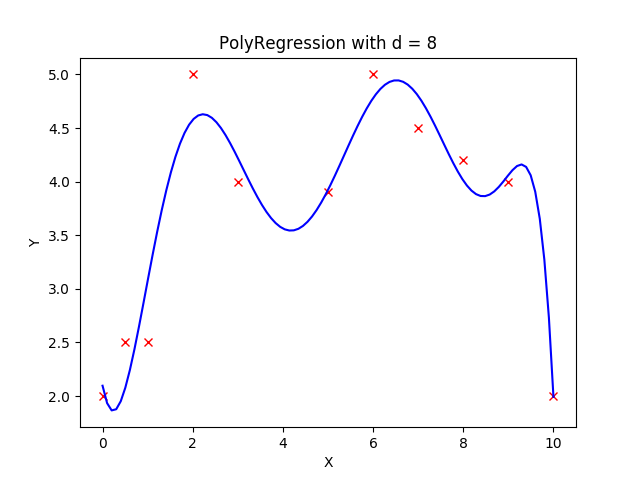
\includegraphics[width=150mm]{../hw1-code/results/a4.png}
\end{figure}

\begin{figure}[!ht]
\centering
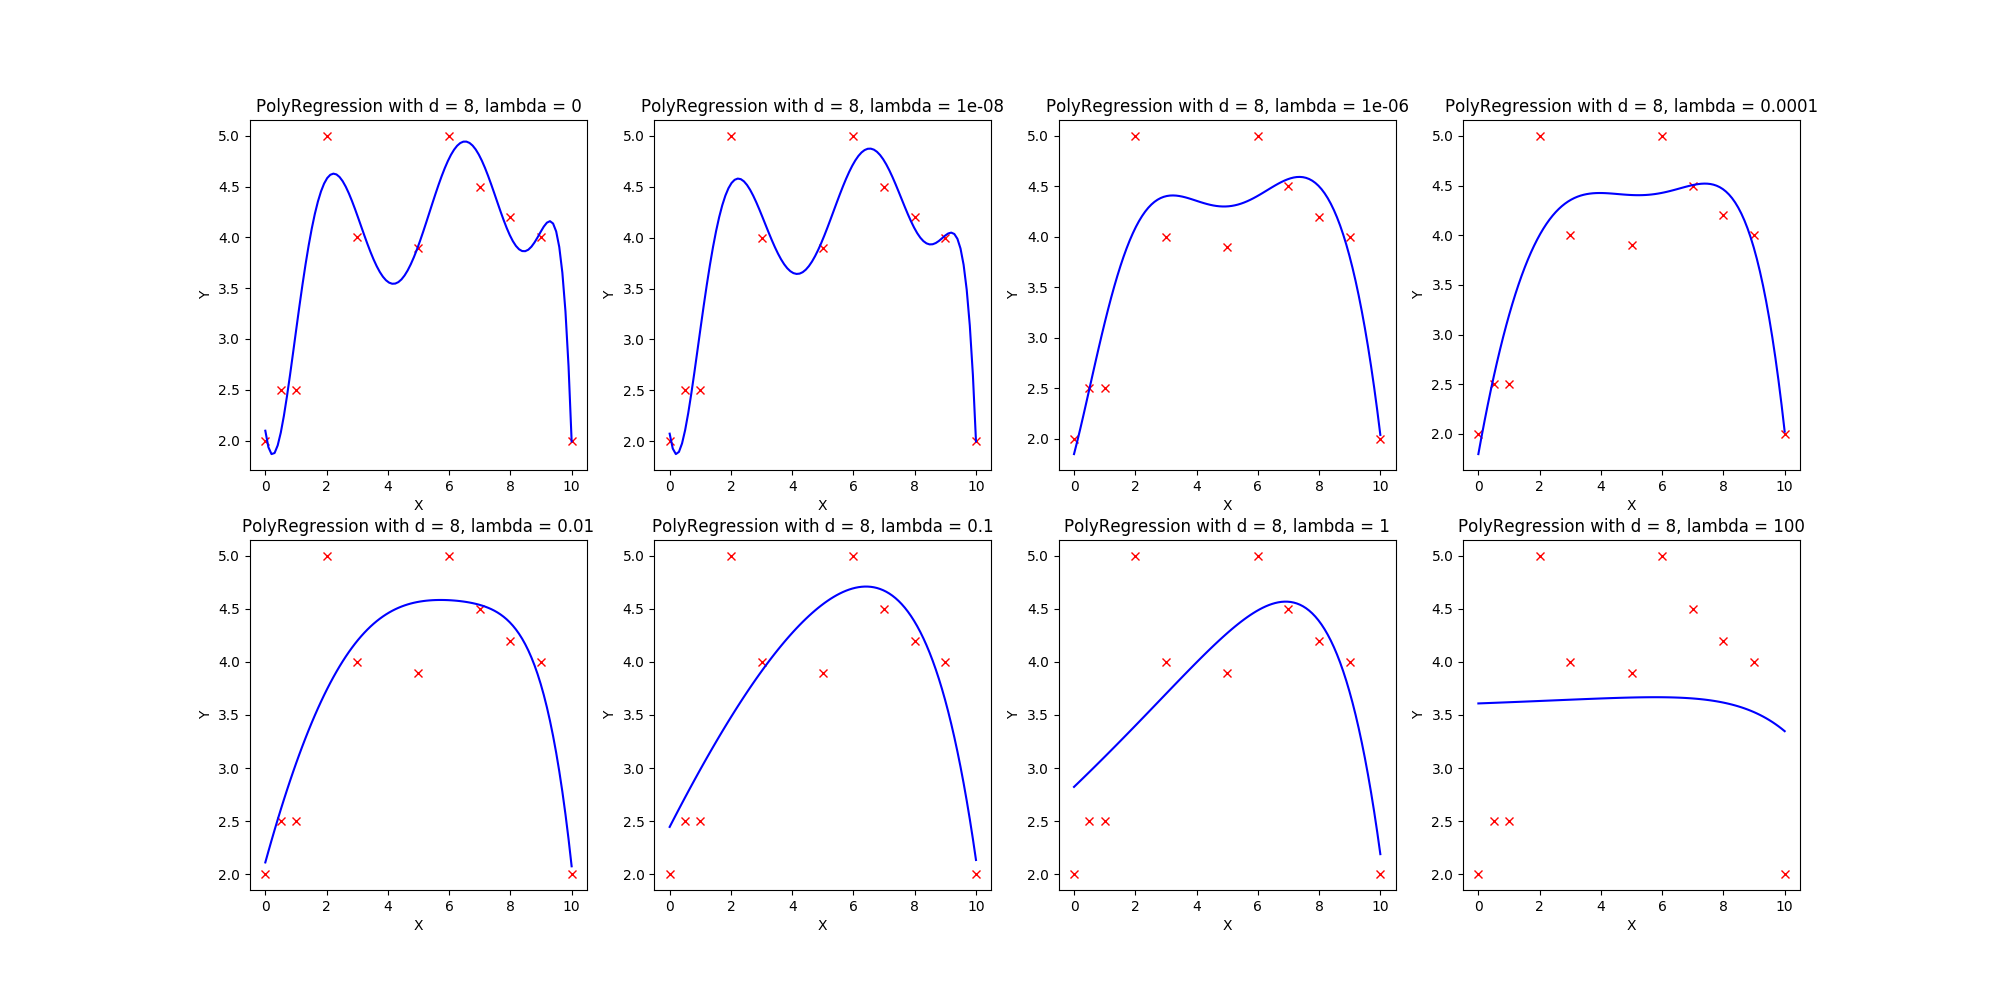
\includegraphics[width=218mm]{../hw1-code/results/a4_compilation.png}
\end{figure}

As lambda increases, we see that the curve seems to smooth out and eventually even flatten out at excessive amounts. There seems to be a good amount of regularization when the curve is relatively smooth with considerably less evidence of overfitting to the specifically selected points around values of 0.01 or 0.1.

\begin{verbatim}
  class PolynomialRegression:

  def __init__(self, degree=1, reg_lambda=1E-8):
      """
      Constructor
      """

      self.degree = degree
      self.reg_lambda = reg_lambda

      self.mean_list = None
      self.std_list = None
      self.theta = None

  def polyfeatures(self, X, degree):
      """
      Expands the given X into an n * d array of polynomial features of
          degree d.

      Returns:
          A n-by-d numpy array, with each row comprising of
          X, X * X, X ** 3, ... up to the dth power of X.
          Note that the returned matrix will not include the zero-th power.

      Arguments:
          X is an n-by-1 column numpy array
          degree is a positive integer
      """
      
      n = len(X)
      d = degree

      result = np.zeros((n, d))

      for i in range(n):
          for j in range(d):
              result[i][j] = X[i] ** (j + 1)

      return result

  def standardize(self, matrix):
      # TODO: check if this is behaving properly
      n, d = matrix.shape

      result = np.zeros((n, d))
      for i in range(d):
          result[:, i] = (matrix[:, i] - self.mean_list[i])
          / self.std_list[i]

      return result


  def fit(self, X, y):
      """
          Trains the model
          Arguments:
              X is a n-by-1 array
              y is an n-by-1 array
          Returns:
              No return value
          Note:
              You need to apply polynomial expansion and scaling
              at first
      """

      n = len(X)
      d = self.degree

      poly_matrix = self.polyfeatures(X, d)
      
      # get the means/stds of training data
      self.mean_list = np.zeros(d)
      self.std_list = np.zeros(d)

      for i in range(d):
          cur = poly_matrix[:, i]
          cur = cur.tolist()

          self.mean_list[i] = np.mean(cur)
          self.std_list[i] = np.std(cur)

      poly_matrix = self.standardize(poly_matrix)

      # add the x0 column of 1s
      poly_matrix = np.concatenate((np.ones((n, 1)), poly_matrix), axis=1)

      # construct reg matrix
      reg_matrix = self.reg_lambda * np.eye(d + 1)
      reg_matrix[0, 0] = 0

      # Since 0-mean, we can do 
      # weight = (X^T*X + r)^-1 X^T*Y
      self.theta = np.linalg.pinv(poly_matrix.T.dot(poly_matrix)
                  + reg_matrix).dot(poly_matrix.T).dot(y)

  def predict(self, X):
      """
      Use the trained model to predict values for each instance in X
      Arguments:
          X is a n-by-1 numpy array
      Returns:
          an n-by-1 numpy array of the predictions
      """

      n = len(X)
      d = self.degree

      poly_matrix = self.polyfeatures(X, d)
      poly_matrix = self.standardize(poly_matrix)

      # add column of 1s at beginning
      poly_matrix = np.concatenate((np.ones((n, 1)), poly_matrix), axis=1)

      # return predictions
      return poly_matrix.dot(self.theta)
\end{verbatim}

% \newpage

% \newpage

}

\section*{A.5}
{\Large 

\begin{figure}[ht!]
  \centering
  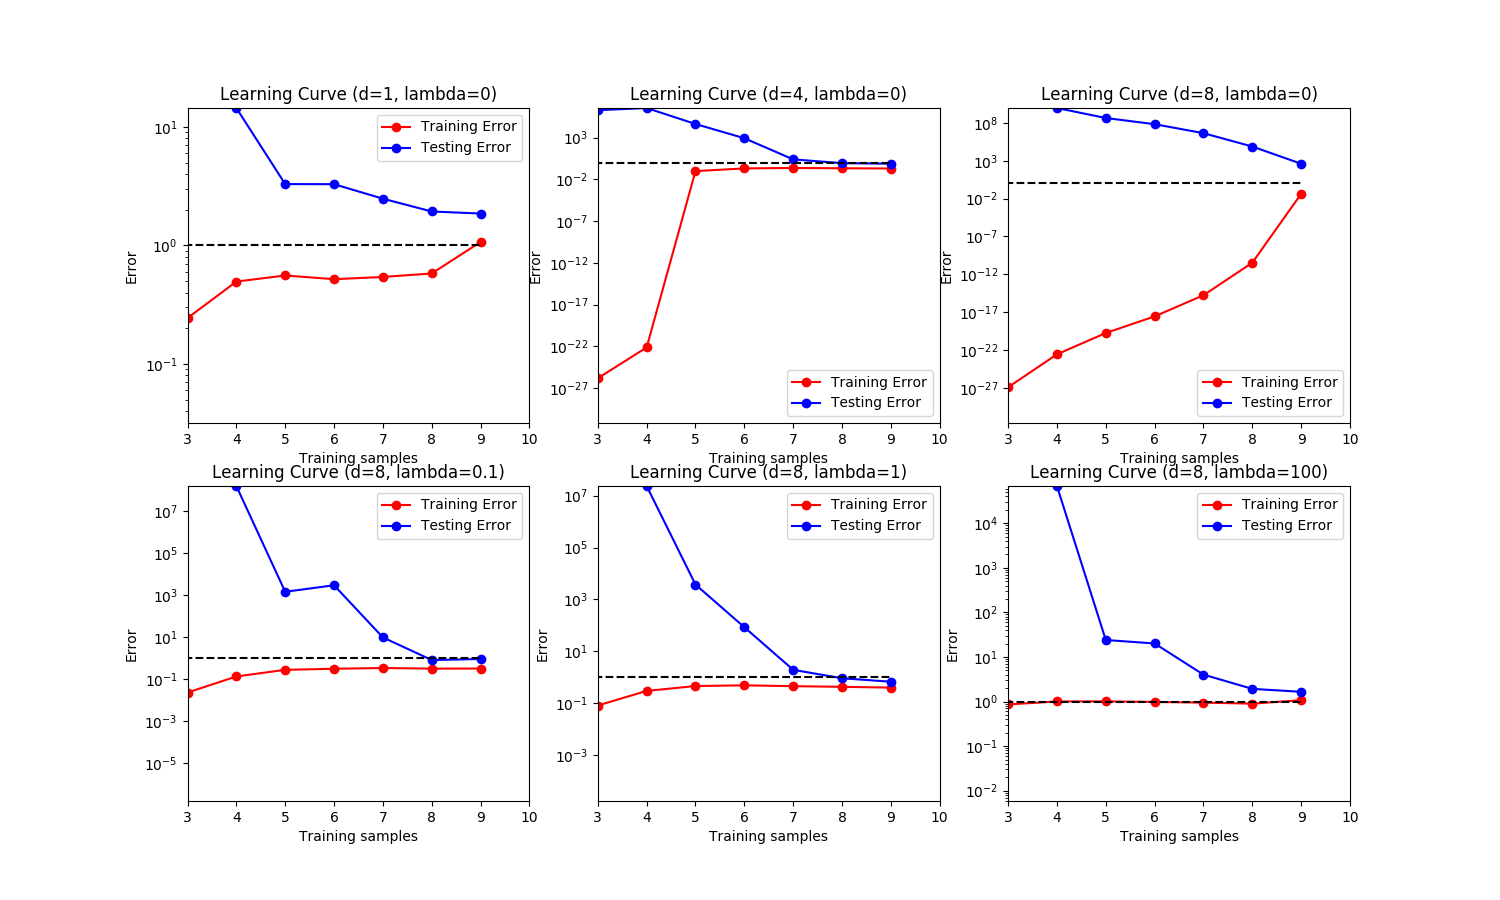
\includegraphics[width=215mm]{../hw1-code/results/a5.png}
\end{figure}

\begin{verbatim}
def calculate_error(n, calculated_values, actual_values):
  result = 0

  for i in range(n):
      result += np.square(calculated_values[i] - actual_values[i])

  return result / n

def learningCurve(Xtrain, Ytrain, Xtest, Ytest, reg_lambda, degree):
  """
  Compute learning curve

  Arguments:
      Xtrain -- Training X, n-by-1 matrix
      Ytrain -- Training y, n-by-1 matrix
      Xtest -- Testing X, m-by-1 matrix
      Ytest -- Testing Y, m-by-1 matrix
      reg_lambda -- regularization factor
      degree -- polynomial degree

  Returns:
      errorTrain -- errorTrain[i] is the training accuracy using
      model trained by Xtrain[0:(i+1)]
      errorTest -- errorTrain[i] is the testing accuracy using
      model trained by Xtrain[0:(i+1)]

  Note:
      errorTrain[0:1] and errorTest[0:1] won't actually matter, since we start displaying the learning curve at n = 2 (or higher)
  """

  n = len(Xtrain)
  m = len(Xtest)

  errorTrain = np.zeros(n)
  errorTest = np.zeros(n)

  #TODO -- complete rest of method; errorTrain and errorTest are already the correct shape

  model = PolynomialRegression(degree, reg_lambda)

  # Xtrain[0 : (i+1)]
  # Ytrain[0: (i+1)]

  for i in range(1, n):
      model.fit(Xtrain[0: (i+1)], Ytrain[0: (i+1)])

      errorTrain[i] = calculate_error(i + 1, model.predict(Xtrain[0: (i+1)]), Ytrain[0: (i+1)])
      errorTest[i] = calculate_error(m, model.predict(Xtest), Ytest)

  return errorTrain, errorTest
\end{verbatim}

% \newpage

}

\section*{A.6}
{\Large 

\subsection*{a.}

We aim to show that $\widehat{W} = (X^TX + \lambda I)^{-1}X^TY$. \\ 
We start with $\widehat{W} = \text{argmin}_{W \in \R^{d \times k}} \sum_{i=1}^{n} \| W^Tx^i - y^i \|_2^2 + \lambda \| W \|_F^2$ \\
To find $\widehat{W}$ using our original form, we take the regularized least squares object and take the gradient with respect to $W$ and set to 0: \\ \\ 
$0 = \nabla_W (\sum_{i=1}^{n} \| W^Tx^i - y^i \|_2^2 + \lambda \| W \|_F^2$) \\
$0 = \nabla_W (\sum_{i=1}^{n} \| W^Tx^i - y^i \|_2^2) + \nabla_W (\lambda \sum_{i=1}^{d}\sum_{j=1}^{k}W_{i,j}^2)$ \\
% i am fucking tripping here
$0 = \nabla_W (\sum_{i=1}^{n} \| W^Tx^i - y^i \|_2^2) + \nabla_W (\lambda I_{ij} W^2)$ \\
$0 = \nabla_W (\sum_{i=1}^{n} \| W^Tx^i - y^i \|_2^2) + 2 \lambda I_{ij} W$ \\
$0 = \nabla_W (\sum_{i=1}^{n} \| x^iW - y^i \|_2^2) + 2 \lambda I_{ij} W$ \\
% think harder about this step
$0 = \nabla_W ((XW - Y)^T(XW - Y)) + 2 \lambda I_{ij} W$ \\
$0 = \nabla_W ((XW)^TXW - (XW)^TY - Y^TXW + Y^TY) + 2 \lambda I_{ij} W$ \\
$0 = \nabla_W (W^TX^TXW - W^TX^TY - Y^TXW + Y^TY) + 2 \lambda I_{ij} W$ \\
$0 = \nabla_W (W^TX^TXW - W^TX^TY - W^TX^TY^T + Y^TY) + 2 \lambda I_{ij} W$ \\
$0 = \nabla_W (W^TX^TXW - 2W^TX^TY + Y^TY) + 2 \lambda I_{ij} W$ \\
$0 = \nabla_W (W^TX^TXW) - 2X^TY + 2 \lambda I_{ij} W$ \\
$0 = X^TXW + W^TX^TX - 2X^TY + 2 \lambda I_{ij} W$ \\
$0 = X^TXW + X^TXW - 2X^TY + 2 \lambda I_{ij} W$ \\
$0 = 2(X^TXW - X^TY + \lambda I_{ij} W)$ \\
$0 = X^TXW - X^TY + \lambda I_{ij} W$ \\
$X^TY = (X^TX + \lambda I_{ij}) W$ \\
$W = (X^TX + \lambda I_{ij})^{-1}X^TY = (X^TX + \lambda I)^{-1}X^TY$ \\
as we aimed to show.

\subsection*{b.}

I divided up my files into mnist\_classifier.py which was my main script, as well as a helper script labeled mnist\_helper.py. I ended up with training error of 0.14801666666666669, or around 14.80\%, and test error of 0.14670000000000005, or around 14.67\%. This can be re-run as desired by simply running "python3 mnist\_classifier.py". \\
The code for mnist\_classifier.py is as follows: \\

\begin{verbatim}
# mnist_classifier.py

import numpy as np
import os
import sys

import mnist_helper as m_h

from scipy import linalg

# Methods

"""
Input: X as n x d, Y as 0/1 n x k, lmbda > 0 as regularization factor
(Modify lmbda in mnist_helper constants)
Output: W-hat predictor
"""
def train(X, Y, lmbda=m_h.lmbda):
  print("train")

  assert (len(X) > 0), "X row count sanity check"

  # d-dimensional since we have (d x n) x (n x d) = d x d
  inverse_term = X.T.dot(X) + (m_h.lmbda * np.eye(len(X[0])))

  return linalg.solve(inverse_term, X.T.dot(Y))

"""
Input: W as d x k, X as m x d
Output: m-length vector with ith entry equal to the maximizer
according to each example from input X
"""
def predict(W, X):
  print("predict")

  return np.argmax(np.dot(X, W), axis=1)

def main(run_type):
  # labels are in list form, ohe are in ohe form
  X_train, labels_train, ohe_train, X_test, labels_test, ohe_test = m_h.load_dataset()

  W_train = train(X_train, ohe_train)
  
  train_predictions = predict(W_train, X_train)
  test_predictions = predict(W_train, X_test)

  train_error = m_h.calculate_error(train_predictions, labels_train)
  test_error = m_h.calculate_error(test_predictions, labels_test)

  print(train_error)
  print(test_error)

if __name__ == '__main__':
  main(sys.argv[1:])

\end{verbatim}
The code for mnist\_helper.py is as follows: \\ 

\begin{verbatim}
# mnist_helper.py

import numpy as np

from mnist import MNIST

# Global Variables

lmbda = 10E-4

n = 0
m = 0

# Helper Functions

"""
Helper function for loading in MNIST data set
"""
def load_dataset():
  mndata = MNIST('../data/')
  X_train, labels_train = map(np.array, mndata.load_training())
  X_test, labels_test = map(np.array, mndata.load_testing())
  X_train = X_train/255.0
  X_test = X_test/255.0

  # convert labels to one-hot encoding
  ohe_train = np.zeros((len(labels_train), 10))
  ohe_test = np.zeros((len(labels_test), 10))

  for idx, train_val in enumerate(labels_train):
    ohe_train[idx][train_val] = 1

  for idx, test_val in enumerate(labels_test):
    ohe_test[idx][test_val] = 1

  return X_train, labels_train, ohe_train, X_test, labels_test, ohe_test

"""
Helper function for calculating the error
"""
def calculate_error(calculated_values, actual_values):
    assert (len(calculated_values) == len(actual_values)
            ), "Equal prediction list length sanity check"
    
    # convert to match boolean list
    match_summary = [calc_val == actual_values[calc_idx]
                     for calc_idx, calc_val in enumerate(calculated_values)]

    return 1 - (sum(match_summary) / len(match_summary))


\end{verbatim}

}

\end{document}